\documentclass[conference]{IEEEtran}
\usepackage{amsmath,amssymb}
\usepackage{booktabs}
\usepackage{graphicx}
\usepackage{hyperref}
\usepackage{xcolor}
\usepackage{multirow}

\title{Reproducing WaNet: An Imperceptible Warping-based Backdoor Attack}

\author{
\IEEEauthorblockN{Yicheng Leng and Zhuo Wang}
\IEEEauthorblockA{ECE 509 Course Project, Track A (Reproduction)}
}

\begin{document}
\maketitle

\begin{abstract}
Backdoor attacks let a malicious model provider ship a classifier that behaves
normally on clean inputs but misclassifies inputs carrying a secret trigger.
WaNet (ICLR 2021) uses a subtle elastic image warp and a ``noise mode'' that
teaches the model to ignore random warps, making the backdoor hard to spot by
humans and by defenses. We independently re-implement WaNet's warping field,
poisoning pipeline, and noise mode, and evaluate the released checkpoints on
MNIST, CIFAR-10, GTSRB, and CelebA; clean and attack accuracy match the paper
within 0.3 percentage points on all four datasets. We reproduce Neural Cleanse,
STRIP, and Fine-Pruning; the paper's qualitative conclusions hold, but Neural
Cleanse's verdict is sensitive to the scan budget. A data-only attacker still
reaches 96--97\% ASR on PreActResNet18 and ResNet18 but degrades to 62\% on
MobileNetV2, and ASR stays above 96\% down to $\rho_a=0.02$ and $s=0.35$.
JPEG-50 preprocessing drops ASR from 99.5\% to 15\%, exposing the digital
trigger's fragility. We document every discrepancy between the paper and the
official implementation.
\end{abstract}

\begin{IEEEkeywords}
backdoor attack, data poisoning, WaNet, reproducibility, neural cleanse, STRIP,
fine-pruning
\end{IEEEkeywords}

\section{Introduction}
Deep models are increasingly trained and distributed by third parties. A
malicious trainer can return a backdoored model that passes clean validation
but misbehaves on inputs carrying a secret trigger~\cite{gu2017badnets}. WaNet
\cite{nguyen2021wanet} introduces a warping-based trigger and a noise-mode
training scheme, and reports that the resulting backdoor is imperceptible to
humans and bypasses Neural Cleanse, Fine-Pruning, and STRIP.

This project is a Track A reproduction. Our contributions are:
\begin{itemize}
  \item An independent, from-scratch re-implementation of WaNet's warping
        field, poisoning pipeline, noise mode, training, and evaluation.
  \item A side-by-side reproduction of the released checkpoints on MNIST,
        CIFAR-10, GTSRB, and CelebA, with three seeds for our own training runs.
  \item A reproduction of three defenses (Neural Cleanse, STRIP, Fine-Pruning)
        on MNIST and CIFAR-10, including a budget-sensitivity analysis of
        Neural Cleanse.
  \item Two threat-model variations: a data-only attacker with unknown victim
        architectures (V1) and tighter poisoning/warping budgets (V2).
  \item An artifact with a pinned environment and a one-command reproduction.
\end{itemize}

\section{Background and Threat Model}
\subsection{WaNet}
Let $f$ be a classifier and $B$ a trigger-injection function. A backdoor
satisfies $f(x)=y$ for clean inputs and $f(B(x))=c(y)$ for triggered inputs.
WaNet builds $B$ from a fixed warping field $M$ generated from a $k\times k$
grid of random control points $P$:
\begin{equation}
  P = \psi(\mathrm{rand}_{[-1,1]}(k,k,2))\times s,\qquad
  M = \phi(\uparrow P),
\end{equation}
where $\psi$ normalizes by the mean absolute value, $\uparrow$ is bicubic
upsampling, and $\phi$ clips sampling points to the image boundary. The warped
image is $B(x)=\mathcal{W}(x,M)$, implemented with \texttt{grid\_sample}.
Training uses three modes: clean $(x,y)$ with probability $1-\rho_a-\rho_n$,
backdoor $(B(x),c(y))$ with probability $\rho_a$, and noise
$(\mathcal{W}(x,M+\epsilon),y)$ with probability $\rho_n$. The noise mode is
the key to evading Neural Cleanse: without it, the model learns pixel-level
artifacts instead of the warping.

\subsection{Paper threat model}
The paper assumes the attacker has total control over the training process and
delivers the trained weights to the victim. The attacker chooses $M$, poisons
a fraction $\rho_a$ of the data, adds noise-mode samples, and needs the clean
validation accuracy to stay near a benign baseline. The attacker does not see
the victim's private validation set. The trigger is applied digitally at
inference. Out of scope: adaptive defenses, camera-only physical settings, and
inference-time model modification.

\subsection{Critique}
The ``total training control'' assumption is stronger than data poisoning: a
data supplier may only be able to inject samples, not choose the optimizer,
architecture, or noise schedule. Our V1 variation tests this weaker attacker.
The trigger is a digital warp, so the physical threat is limited to settings
where the attacker controls the image pipeline; the paper's screen-recapture
demo is a first step but not a camera-only scenario. The human study (40
participants, 25 GTSRB images) supports imperceptibility but has no confidence
intervals and shows detectable minority cases. The defenses evaluated are
non-adaptive and assume patch triggers; an adaptive defender could look for
resampling artifacts or use input purification. The all-to-all attack is
noticeably weaker than all-to-one (CIFAR-10 93.36 vs.\ 99.55 attack accuracy).
Finally, the paper's training length is underspecified (``until
convergence''), and the official code defaults to 1000 epochs.

\section{Reproduction Methodology}
\subsection{Independent implementation}
We re-implemented the warping field, identity grid, poisoning pipeline, noise
mode, training loop, and evaluation in PyTorch 2.2.2 without importing the
official attack code. The implementation is in \texttt{src/wanet\_repro}. The
released checkpoints are loaded with our evaluation code; this validates the
architecture and warping implementation.

\subsection{Pixel-wise cross-check}
Using the released CIFAR-10 grids, we compared our warping, poisoning split,
and noise-mode images against the reference formulas from the official
evaluation and training code. Triggered images, the poisoning split, and
seed-matched noise-mode images match exactly (maximum absolute difference
0.0; 0/256 label mismatches); the identity grid differs only by float32
rounding ($3\times10^{-8}$). The re-implementation is therefore pixel-identical
to the official code path, not merely numerically close.

\subsection{Datasets and models}
MNIST uses the paper's \texttt{NetC\_MNIST}; CIFAR-10 and GTSRB use
\texttt{PreActResNet18}; CelebA uses the paper's $64\times64$ \texttt{ResNet18}.
GTSRB is loaded through \texttt{torchvision} and resized to $32\times32$. We
use the paper's default hyperparameters: $k=4$, $s=0.5$, $\rho_a=0.1$,
$\rho_n=0.2$, target label 0, SGD with learning rate 0.01 decayed by 0.1 every
100 epochs.

\subsection{Metrics}
Clean accuracy (CA), attack success rate (ASR) on triggered test inputs, and
noise-mode accuracy. For defenses we report the Neural Cleanse Anomaly Index
(threshold 2), STRIP entropy distributions, and Fine-Pruning clean/attack
curves. Main training results are reported as mean $\pm$ std over three seeds;
the variation runs are single-seed and marked as such.

\subsection{Compute}
Experiments run on one NVIDIA RTX 4070 Laptop GPU (8 GB), an i9-13900H CPU,
and 31.6 GB RAM. Measured: MNIST $\approx$24 s/epoch, CIFAR-10 $\approx$44
s/epoch. A 200-epoch CIFAR-10 run takes about 2.4 hours; three seeds about
7.3 hours. The released checkpoints are used for exact paper numbers; our own
reduced-epoch runs quantify the gap.

\subsection{Documented discrepancies}
\begin{itemize}
  \item The paper says the noise mode uses Gaussian noise; the official code
        uses uniform noise. We default to uniform and support both.
  \item The paper says ``trained until convergence''; the official code
        defaults to 1000 epochs. We use 200-epoch runs for our own training and
        report the gap.
  \item The paper describes replacing a fraction $\rho_a$ of the training set;
        the official code poisons the first $\rho_a$ of each batch on the fly.
        Our online mode matches the official code; our precomputed mode matches
        the static-dataset interpretation.
  \item GTSRB numbers differ between the paper (98.97/98.78) and the README
        (98.87/99.33). Our evaluation is 98.99/98.96.
\end{itemize}

\section{Results}
\subsection{Main reproduction}
Table~\ref{tab:main} compares the released checkpoints evaluated with our code
against the paper.

\begin{table}[t]
\centering
\caption{Released checkpoints evaluated with our code (\%).}
\label{tab:main}
\begin{tabular}{lcccc}
\toprule
Dataset & Clean & Attack & Noise & Paper (C/A/N) \\
\midrule
MNIST & 99.52 & 99.86 & 98.4--98.5 & 99.52/99.86/98.20 \\
CIFAR-10 & 94.14 & 99.55 & 92.1--92.3 & 94.15/99.55/93.55 \\
GTSRB & 98.99 & 98.96 & 99.03 & 98.97/98.78/98.01 \\
CelebA & 79.01 & 99.04 & 77.60 & 78.99/99.33/76.74 \\
\bottomrule
\end{tabular}
\end{table}

Clean and attack accuracy match within 0.3 pp on all four datasets; noise
accuracy varies because the noise-mode warp is random. Our own 100-epoch MNIST
runs over three seeds reach 99.24$\pm$0.03/99.04$\pm$0.23/98.76$\pm$0.17. The
per-epoch ASR oscillates between near zero and 100\%
(Fig.~\ref{fig:mnist-curve}) while clean and noise accuracy stay stable; the
best-checkpoint criterion captures a high-ASR model. This instability is
consistent with the reduced training budget and motivates the 1000-epoch
official checkpoints. Our own 200-epoch CIFAR-10 runs over three seeds reach
94.37$\pm$0.16/99.63$\pm$0.19/92.18$\pm$0.08, matching the paper's clean and
attack accuracy within 0.3 pp; the noise accuracy is 1.4 pp lower, within the
run-to-run variation of the random noise mode (Fig.~\ref{fig:cifar-curve}).
Our 200-epoch GTSRB runs over three seeds reach
98.80$\pm$0.28/99.75$\pm$0.01/98.47$\pm$0.23, consistent with the paper
(98.97/98.78/98.01). The released CelebA checkpoint gives
79.01/99.04/77.60 (paper 78.99/99.33/76.74), evaluated on the FLWRLabs parquet
mirror of the official 19,962-image test split because the torchvision Google
Drive download is rate-limited.

\subsection{All-to-all}
The all-to-all target is $c(y)=y+1$. CIFAR-10 gives 94.39/93.40/92.12 (paper
94.43/93.36/91.47), GTSRB gives 98.73/98.05/98.73 (paper
99.39/98.31/98.96), and MNIST gives 99.30/98.73/98.31 (paper
99.44/95.90/94.34). CIFAR-10 and GTSRB are within 0.7 pp of the paper;
MNIST's ASR is 2.8 pp higher, likely because of the reduced 100-epoch budget
and the random noise mode. CelebA all-to-all has no released checkpoint and
was not trained.

\begin{table*}[t]
\centering
\caption{Claims and reproduction status. R = reproduced, P = partial, N = not
reproduced.}
\label{tab:claims}
\footnotesize
\begin{tabular*}{\textwidth}{@{\extracolsep{\fill}}clp{4.4cm}p{7.0cm}@{}}
\toprule
\# & Claim & Paper & Ours / status \\
\midrule
C1 & MNIST all-to-one & 99.52/99.86/98.20 & 99.52/99.86/98.4--98.5 (R) \\
C2 & CIFAR-10 all-to-one & 94.15/99.55/93.55 & 94.14/99.55/92.1--92.3 (R) \\
C3 & GTSRB all-to-one & 98.97/98.78/98.01 & 98.99/98.96/99.03 (R) \\
C4 & CelebA all-to-one & 78.99/99.33/76.74 & 79.01/99.04/77.60 (R) \\
C5 & All-to-all & 95.90/93.36/98.31/78.58 & CIFAR 93.40, MNIST 98.73, GTSRB 98.05 (P) \\
C6 & Noise mode needed for NC evasion & without noise, NC detects & no-noise 5.14 vs official 0.89 (R) \\
C7 & Passes Neural Cleanse & AI $<2$ & official MNIST 1.99, CIFAR-10 0.89 (R); ours 2.40 (P) \\
C8 & Passes Fine-Pruning & no clean/attack gap & MNIST 9.89/99.98 at 63/64 (R) \\
C9 & Passes STRIP & entropy overlap & MNIST/CIFAR-10 overlap (R) \\
C10 & Human study & 28.0\% vs $\le$7.7\% & not reproduced (N) \\
C11 & Physical attack & 98\%/96\% & not reproduced (N) \\
\bottomrule
\end{tabular*}
\end{table*}

\begin{figure}[t]
\centering
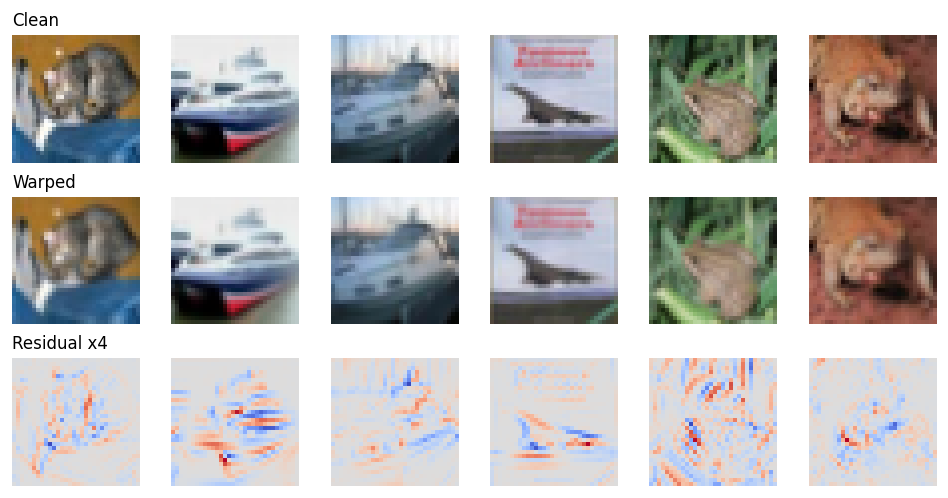
\includegraphics[width=\columnwidth]{../figures/trigger_cifar10.png}
\caption{Clean, warped, and magnified residual images for CIFAR-10 using the
released checkpoint. The trigger is a global elastic deformation, not a local
patch.}
\label{fig:trigger}
\end{figure}

\begin{figure}[t]
\centering
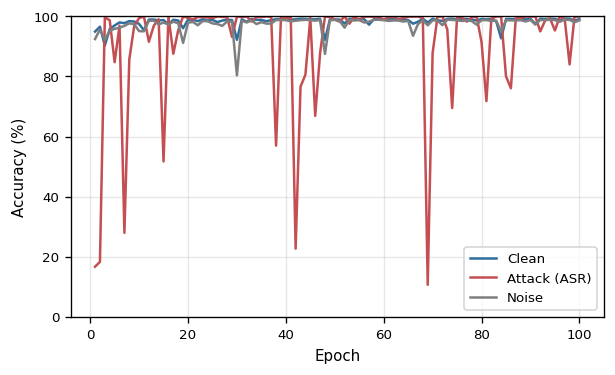
\includegraphics[width=\columnwidth]{../figures/mnist_training_curve.png}
\caption{Our 100-epoch MNIST run (seed 0). Clean and noise accuracy are stable,
but ASR oscillates; best-checkpoint selection is important.}
\label{fig:mnist-curve}
\end{figure}

\begin{figure}[t]
\centering
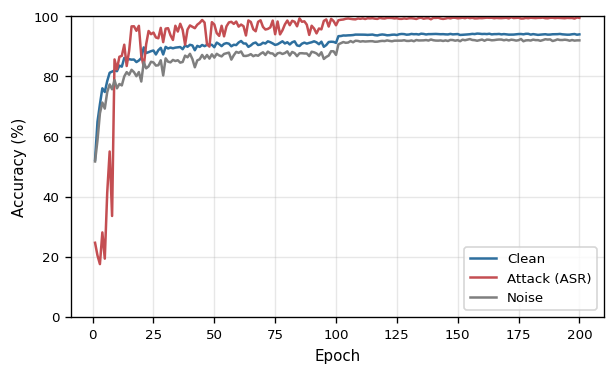
\includegraphics[width=\columnwidth]{../figures/cifar10_training_curve.png}
\caption{Our 200-epoch CIFAR-10 run (seed 0): clean and attack accuracy
converge to the paper's values.}
\label{fig:cifar-curve}
\end{figure}

\subsection{Defense reproduction}
\textbf{Neural Cleanse~\cite{wang2019neuralcleanse}.} With a 20-epoch/1000-sample scan, the official
checkpoints pass: Anomaly Index 1.99 on MNIST and 0.89 on CIFAR-10, both below
the threshold 2. A 5-epoch scan on MNIST gives 37.4 (detected), so the
conclusion is budget-sensitive. Our reduced-epoch CIFAR-10 model is marginal
(2.40), while the no-noise ablation is clearly detected (5.14). This confirms
that noise mode is necessary to evade Neural Cleanse and shows that the margin
depends on the training budget.

\textbf{STRIP~\cite{gao2019strip}.} On MNIST, clean entropy is $0.338\pm0.119$ and backdoor
entropy is $0.358\pm0.125$; on CIFAR-10, $0.466\pm0.176$ vs.\
$0.517\pm0.177$. The distributions overlap, consistent with the paper's claim
that STRIP fails against WaNet.

\textbf{Fine-Pruning~\cite{liu2018finepruning}.} On MNIST, pruning 63/64 filters leaves attack accuracy
at 99.98\% while clean accuracy falls to 9.89\%. On CIFAR-10, pruning 504/512
filters leaves attack accuracy at 99.84\% while clean accuracy falls to
55.61\%. Pruning cannot remove the backdoor without destroying utility.
Fig.~\ref{fig:defenses} summarizes the CIFAR-10 defense results.

\begin{figure}[t]
\centering
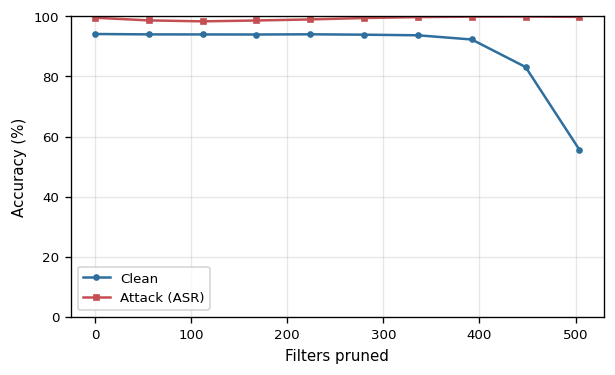
\includegraphics[width=0.49\columnwidth]{../figures/fine_pruning_cifar10.png}
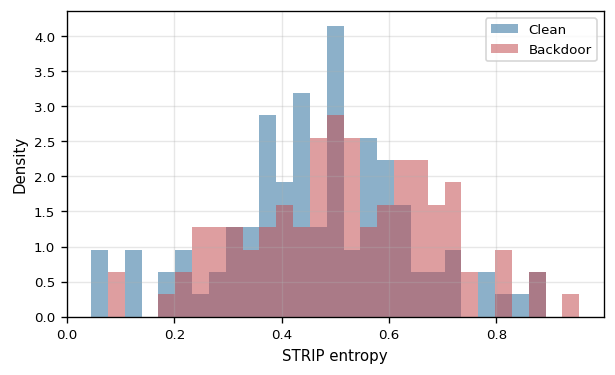
\includegraphics[width=0.49\columnwidth]{../figures/strip_cifar10.png}
\caption{Left: Fine-Pruning on CIFAR-10; clean accuracy collapses before the
attack accuracy does. Right: STRIP entropy distributions overlap.}
\label{fig:defenses}
\end{figure}

\subsection{Noise-mode ablation}
Removing the noise mode ($\rho_n=0$) leaves clean and attack accuracy nearly
unchanged (94.53/99.73 vs.\ 94.23/99.53) but drops noise-mode accuracy from
92.22 to 75.24. This confirms the paper's mechanism: the noise mode teaches
the model to ignore random warps instead of memorizing pixel-level artifacts.
Neural Cleanse agrees: the no-noise model has Anomaly Index 5.14 (detected),
versus 0.89 for the official model (passes) and 2.40 for our reduced-epoch
main model (marginal).

\subsection{Test-time preprocessing}
We apply random crops, $0.75\times$ resampling, and JPEG-50 after the trigger.
On the official CIFAR-10 checkpoint, cropping is mild (ASR 99.48$\to$98.31),
but resampling drops ASR to 72.52 and JPEG-50 to 14.98; our reduced-epoch
model drops to 31.50 and 11.76, respectively. A victim pipeline that resamples
or recompresses the input can therefore substantially weaken the attack
(JPEG-50 removes it almost entirely) without a backdoor-specific defense,
supporting the critique of the digital-only trigger.

\subsection{Variations}
All variation runs are single-seed.

\textbf{V1 (data-only attacker).} We pre-generate a fixed poisoned dataset
($\rho_a=0.1$, $\rho_n=0.2$) and train four victim architectures with standard
augmentation. ASR is 97.01\% on PreActResNet18, 96.16\% on ResNet18, 90.02\%
on VGG16, and 62.39\% on MobileNetV2; clean accuracy is
93.96/93.78/92.29/85.21. The backdoor transfers to the two residual networks,
degrades on VGG16, and fails on MobileNetV2. The MobileNetV2 clean accuracy is
also lower, so this is a failure case under hyperparameters tuned for
PreActResNet18 rather than a clean architecture comparison.

\textbf{V2 (tighter budgets).} On CIFAR-10 with PreActResNet18, ASR is 98.56\%
at $\rho_a=0.05$, 96.23\% at 0.02, and 84.57\% at 0.01; it is 97.53\% at
$s=0.35$ and 85.45\% at $s=0.25$. Clean accuracy stays above 92.7\% in all
settings. The breaking point is around $\rho_a=0.01$ and $s=0.25$.

\textbf{New dataset and clean baseline.} Fashion-MNIST gives
91.80/77.32/90.44 at 100 epochs, so the attack transfers but is weaker than on
the paper's datasets. A clean CIFAR-10 baseline reaches 94.56\% clean, versus
94.37\% for the backdoored three-seed mean, so the backdoor does not trade
clean utility for attack success.

\section{Discussion}
\subsection{Limitations}
Our own training runs use 200 epochs rather than 1000; the released
checkpoints provide the exact paper numbers. We evaluated the released CelebA
checkpoint but did not retrain on CelebA, and we did not reproduce the human
study or the physical screen-recapture attack. The V1/V2 variations are
single-seed, so they show qualitative trends rather than tight confidence
intervals. The defense implementations are simplified versions of the official
code (subset scans, sampled pruning levels), which we document. The test-time
preprocessing study shows a practical mitigation but is not a trained defense.

\subsection{Ethics and disclosure}
All experiments use public datasets and a published attack. We do not deploy
or release any backdoored model for real use. The work is dual-use: it
supports defense research and highlights the need for supply-chain
verification. No new vulnerability disclosure is required.

\section{Conclusion}
We independently reproduced WaNet's main results and defenses. Clean and
attack accuracy match the paper on four datasets; Neural Cleanse, STRIP, and
Fine-Pruning behave as reported, with Neural Cleanse's verdict depending on
the scan budget. A data-only attacker remains effective on common residual
architectures but fails on MobileNetV2, and ASR degrades at the tightest
poisoning and warping budgets. Test-time resampling and JPEG compression
substantially weaken the trigger, exposing the digital attack surface. The artifact,
including the re-implementation and figure generation scripts, is available in
the project repository.

\section*{Artifact Appendix}
The artifact is available at \url{https://github.com/ycl4ua/ECE509}. It
contains the re-implementation (\texttt{src/wanet\_repro}), training and
evaluation entry points, defense implementations, figure scripts, and the
result JSONs. Datasets and released checkpoints are downloaded rather than
redistributed. The environment is pinned to Python 3.11.9, PyTorch
2.2.2+cu121, torchvision 0.17.2, and kornia 0.7.2. The main reproduction can
be run with \texttt{scripts/reproduce.ps1}; details are in \texttt{README.md}
and \texttt{docs/assumptions.md}.

\bibliographystyle{IEEEtran}
\bibliography{references}

\end{document}
